\chapter{Methods for IACT Analyses}
warum brauchen wir das und ach ja jetzt folgt das

\section{Coordinate Frames}

\section{Monte Carlo Simulations}
Today monte carlo simulations are a crucial part to 
understand the behaviour of an experiment. 
Simulating the underlying physic and the response of the experiment
allows the testing of new algorithms aswell as improving the general understanding
of the physical processes at work. Since simulations are always based on our 
current level of understanding, any difference to the measured data
points towards insufficient understanding of the underlying processes.

In CTA monte carlo simulations are done using a combination of the
programs CORSIKA and sim\_telarray

\subsection{Air Shower Simulation with CORSIKA}
CORSIKA \cite{heck1998corsika} is the standard program to simulate different types of
air showers. It allows to choose primary particles at will and
propagate them through the atmosphere, generating secondary particles, until
eventually the ground is reached.
Simulation options include, amongst other:
\begin{itemize}
  \item amount of data to simulate
  \item several random seeds
  \item primary particle type
  \item range and slope of the energy spectrum
  \item alt/az range
  \item models and parameters for the electromagnetic and hadronic interactions
  \item models and parameters for the cherenkov light generation
  \item atmospheric properties, such as the magnetic field
  \item position and size of the detector grid
\end{itemize}

\subsection{Detector Simulation with sim\_telarray}
While CORSIKA handels the formation and propagation of air showers,
the detector response can be simulated using the software
sim\_telarray \cite{BERNLOHR2008149}.

\section{CTA's processing pipeline: ctapipe}
was ist ctapipe?
welcher stand? -> was nutze ich
ctapipe kann schon viel.
eine analyse mit ctapipe sieht dann so aus
\subsection{Low Level Processing}

\subsection{high level}
\subsection{hillas reconstructor}

\section{unser ersatz für missing ctapipe stuff}
\subsection{disp methode}
\subsection{random forests}
das ist supervised und das macht man so:

%\section{Supervised learning}
In the task of supervised machine learning a model is trained on a
dataset with full information available.
This data will come from Monte Carlo simulations in our case, but
could also be e.g. historical or hand labeled datasets in other contexts.
The trained model can then later be used to estimate features on a dataset, which
lacks the needed information.

We define a dataset as having a number of samples with a fixed number of
variables (features) each.
In the following we split
the features of our dataset into a set of \textbf{input} variables $X$ and
a set of \textbf{output} variables $y$.

The naming convention for
these sets follows the one of scikit-learn
\cite{scikit-learn}, \cite{sklearn_api}, a python package for
machine learning algorithm.
We will later use scikit-learn as a basis to train our machine learning models.
Other terminologies for the two feature sets include
predictors or independent variables for the input, and
responses or dependent variables for the output.

Methods based on Decision Trees work by recursively partitioning
the parameter space until the remaining samples behave similar enough.
Tree-based methods can be applied to both classification and regression tasks.

Forest methods combine multiple tree predictors to get more stable
predictions.

\subsubsection{Classification}
In (supervised) classification tasks, we want to predict of which of some
predefined classes the given sample is a member. The possible solutions for $y$
are from a discrete set of values in
contrast to a regression problem with a continuous solution space.
A model that performs classification on data is referred to as a
classifier.

The simplest and most popular case of classification problems
is \textbf{binary classification} \cite{sokolova2009systematic}.
In this case only two distinct
classes exist, which fortunately is all we will need for
our signal/background-separation.
A common example for a classification problem is an Email spam filter,
where mails get categorized in at least two categories based
on their content and meta data \cite{DBLP:journals/corr/cs-CL-0006013}.

For binary classification we can define a set of measures
to define the quality of our prediction, starting with the confusion matrix
shown in table \ref{tab:confusion},
with $pos$ referring to the true label of the positive (i.e. signal)
and $neg$ referring to the label of the negative (i.e. background) class.

\begin{table}
    \caption{Definition of a confusion matrix for binary classification.
    The main diagonal includes the correct predictions, wrong predictions are on the off diagonal.}
    \begin{center}
        \begin{tabular}{ l| l l}
            %\hline
            {} & Predicted as $pos$ & Predicted as $neg$ \\
            \hline
            $pos$ & true positive ($tp$) & false negative ($fn$) \\
            %\hline
            $neg$ & false positive ($fp$) & true negative ($tn$) \\
            %\hline
        \end{tabular}
    \end{center}
    \label{tab:confusion}
\end{table}

An ideal classification would result in
\begin{equation*}
  fp = fn = 0.
\end{equation*}

Based on the confusion matrix, multiple measures
can be constructed to examine the classifiers performance.
Some of the more common ones are listed in table \ref{tab:class_metrics}.

\begin{table}
    \caption{Popular metrics for binary classification tasks.}
    \begin{center}
        %\caption{
         % Common metrics for classification tasks, taken from \cite{sokolova2009systematic}.}
        \begin{tabularx}{\textwidth}{l c X}
            %\hline
            Measure & Formula & Interpretation \\
            \hline
            Accuracy & $\frac{tp+tn}{tp+fn+fp+tn}$ & Overall effectiveness of a classifier \\
            %\hline
            Precision & $\frac{tp}{tp+fp}$ & Class agreement with the positive labels given by the classifier \\
            %\hline
            Recall/Sensitivity & $\frac{tp}{tp+fn}$ & Effectiveness of a classifier to identify positive labels \\
            %\hline
            F$_{\beta}$-score & $\frac{(\beta^2+1)tp}{(\beta^2+1)tp+\beta^2fn+fp}$ & Harmonic mean between precision and recall with choosable $\beta$ \\
            %\hline
            Specificity & $\frac{tn}{fp+tn}$ & How effectively a classifier identifies negative labels \\
            %\hline
            Balanced Accuracy & $\frac{1}{2}(\frac{tp}{tp+fn}+\frac{tn}{fp+tn})$ & Classifier’s ability to avoid false classification \\
        %\hline
        \end{tabularx}
        %\caption{Overview of common metrics for classification tasks based on the
        %intermediate metrics shown in table \ref{tab:confusion}}
    \end{center}
    \label{tab:class_metrics}
\end{table}

We will make use of the precision, recall and F-score.
Additionally we will calculate the Area Under the Curve (AUC) with regard to the Receiver Operating Characteristic (ROC) curve.
The ROC-curve is gained by plotting the true positive rate against the false positive rate while varying the classifier threshold.
The area under the (normalised) ROC-curve is thus a measure for whether the classifier will
rank a randomly chosen positive sample higher than a randomly chosen negative sample \cite{FAWCETT2006861}.

\subsubsection{Regression}
Regression is the task of predicting a continuous variable
from a set of input variables.
The simplest approach
to this problem is the ordinary linear least squares method.

Given an unrestricted linear model
\begin{align}
	y &= X\beta + e \\
	E(y) &= X\beta \\
	Cov(y) &= \sigma^2 I_n
\end{align}
with a measured vector $y$, the design matrix $X$,
an unknown parameter vector $\beta$, a random error $e$
and pairwise orthogonal features $y_i$,
the least-squares solution is given by the solution of
the minimizing problem in equation \ref{eq:min_least_squares}.

\begin{equation}
	\min_{\beta\in\mathbb{R}^k} \lVert y - X\beta \rVert
	\label{eq:min_least_squares}
\end{equation}

If $(X^TX)^{-1}$ exists, the unique solution for the
least square estimation of $\beta$ becomes:
\begin{equation}
	\hat{\beta} = X^+ y,
\end{equation}

with the Moore-Penrose inverse $X^+ = (X^TX)^{-1}X^T$.
The estimation of $y$ then becomes:
\begin{equation}
  \hat{y} = X\hat{\beta}.
\end{equation}

The metric, that is minimized by the least-squares solution
is the Mean Squared Error (MSE).

Other metrics for regression tasks include the
Root-Mean-Squared-Error(RMSE),
Mean-Absolute-Error(MAE)
or the Coefficient of Determination ($R^2$), all of which are listed in table
\ref{tab:regr_metrics}.

\begin{table}
  \caption{Popular metrics for a regression problem with $n$ samples.}
  \begin{center}
    \begin{tabularx}{\textwidth}{l c X}
      Measure & Formula & Interpretation \\
      \hline
      Mean squared error & $\frac{1}{n}\sum_i^n |y_i-\hat{y_i}|$ & Prediction error disregarding the direction of over- and underprediction \\
      Mean absolute error & $\frac{1}{n}\sum_i^n (y_i-\hat{y_i})^2$ & For an unbiased predictor: Variance of the regressor. Heavily weights outliers. \\
      Coefficent of Determination & $1 - \frac{\sum_i^n (\bar{y_i}-\bar{y})^2}{\sum_i^n (y_i-\bar{y})^2}$ & Share of observed variance that is explained by the model.\\
    \end{tabularx}
  \end{center}
  \label{tab:regr_metrics}
\end{table}

Many metrics closely connected to these metrics exist, such as root mean squared error (RMSE)
or the mean absolute percentage error (MAPE).
Our analysis will be based on the use of the MSE.

\subsubsection{From Decision Trees to Random Forests}
A simple (binary) decision tree
for an example classification on the iris dataset
is shown in figure \ref{fig:03_tree}.

\begin{figure}
  \centering
  \captionsetup{width=0.9\linewidth}
  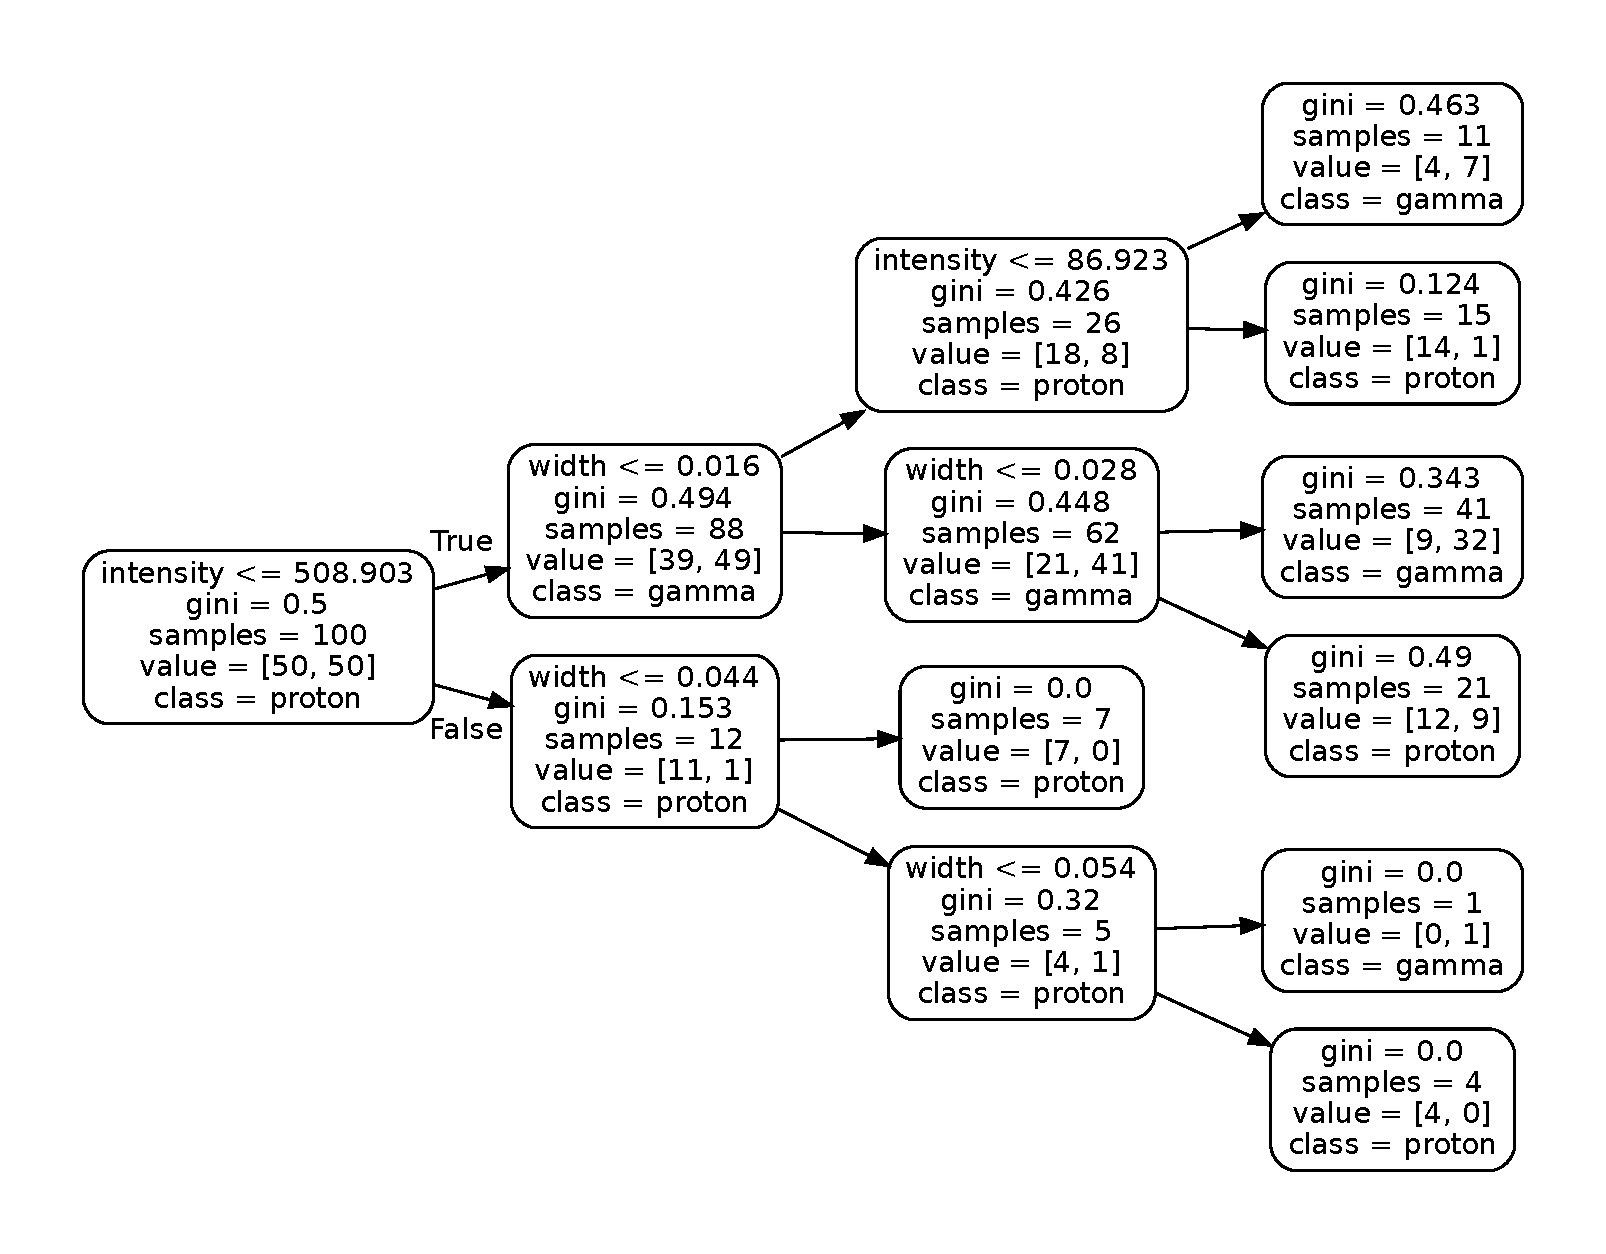
\includegraphics[width=0.9\textwidth]{Plots/decision_tree.pdf}
  \caption{A very simple decision tree for demonstrational purposes.
      The dataset in use is the famous iris dataset that includes
      measurements of the petal and sepal width and length
      for three different flower classes \cite{fisher1936use}.
      Each node lists (from top to bottom): The cut that will
      be applied with the samples fulfilling the condition going
      into the left node and the remaining samples in the right node.
      The gini coefficient evaluated on the associated samples.
      Once it reaches zero, no further splits are performed.
      The number of samples that ended up in the node and last the
      class distribution in the samples.
      One can derive that the first class can immediately be separated from
      the other two classes (left node, first split), while the other two classes
      are harder to separate and require multiple cuts for a perfect separation.}
  \label{fig:03_tree}
\end{figure}

Starting from the root node, a binary split is performed to
split up the data. For each resulting node additional splits are performed
until a stopping criterion is reached.
Choosing the optimal split is defined as minimizing a
pre-defined measure.

For classification tasks this means reducing the class impurity in the node.
Often used measures
to quantify the impurity are gini coefficient, that is used in the example, or the
cross-entropy \cite{hastie2017springer}.
Both are defined in equation \ref{eq:gini_ce}

\begin{align}
	\text{Gini impurity: } &= \sum_{k=1}^K \hat{p}_{mk}(1-\hat{p}_{mk}) \\
	\text{Cross-entropy: } &= -\sum_{k=1}^K \hat{p}_{mk}\log{\hat{p}_{mk}},
  \label{eq:gini_ce}
\end{align}

with $p_{mk}$ denoting the proportion of class $k$ in node $m$.

A stopping criterion can be defined as the measure reaching a
a defined threshold or not improving anymore.
Alternatively the tree can stop at a predefined depth to
avoid overly complex models.

For regression tasks scikit-learn uses the mean squared error
or mean absolute error and the same principles apply.
We will later use the Gini impurity and the Mean Squared Error
for the classification and regression tasks respectively.

The implementation in sklearn is based on the one by
Leo Breiman et al \cite{breimanclassification}.
A single tree performs binary splits $\Theta = (j, t_m)$
at each node $m$ in order to split
the data at this node $Q$ into two subsets
$Q_\text{left}$
and
$Q_\text{right}$.
The split consists of a feature $j$ and a threshold $t_m$ and is
chosen in a way to minimize the given measure.
Features, that are more important for the task, will
thus appear at the top nodes of the tree.


While decision trees have the benefit of providing
easily interpretable, low bias models there are some drawbacks to this
approach, namely \cite{hastie2017springer}:
\begin{itemize}
  \item{Instability, high variance}
  \item{Lack of Smoothness}
  \item{Difficulty in Capturing Additive Structure}.
\end{itemize}

Approaches to reducing these problems include
boosting \cite{freund1997decision} and Random Forests \cite{Breiman2001}.

Überleitung!

Random forests have become one of the standard algorithms
in data analysis tasks, because according to our
experience and \cite{hastie2017springer} they tend to
rarely overfit (as long as the individual trees have no or little bias)
and generally perform decent without a lot of manual tuning.

The main idea behind random forests is to use multiple, independent
decision trees to suppress the problems single trees have, while
keeping their advantages.
For this to work, the individual trees need not to be correlated.
Consequently the trees cannot all be constructed the same way.
To make sure the individual trees
- and their predictions -
are somewhat independent from each other,
some kind of randomness has to be introduced to the tree.
In random forests this is on the one hand achieved by giving each tree a
randomly drawn subsample from the training data.
This is referred to as bootstrapping \cite{efron1992bootstrap}.
Another source of randomness is to perform splits on a node
based on only a random subsample of the available features.

The prediction of the random forest in scikit learn is then the average of
the single trees predictions.
In the case of a classification task, the probabilistic predictions for each class
get averaged.